\section{Modulübersicht} \label{app:modul}
Die App besteht aus fünf Modulen, die sich gemäß MVP einer der Rollen Model, View oder Presenter zuordnen lassen. Dabei unterteilen sich komplexere Module in weitere Unterpakete. Die View-Rolle übernimmt das Gui Modul~\eqref{app:module:gui} zusammen mit den XML-Layout Dateien. Die Presenter-Rolle wird durch das ApplicationLogic Modul~\eqref{app:module:applicationlogic} realisiert. Das Utils-Modul~\eqref{app:module:utils} unterstützt es dabei mit grundlegenden Operationen und Datenstrukturen. Als Model agiert das Modul Data~\eqref{app:module:data}. Schaubild \ref{fig:modules_overview} veranschaulicht die Einteilung:
\begin{figure}[ht]
	\centering
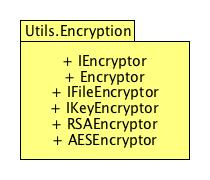
\includegraphics[width=1\textwidth]{./resources/Diagramme/App/modules_overview.jpg}
\caption{Module der Android App}
	\label{fig:modules_overview}
\end{figure}
\label{app:module:gui}\subsection{Gui}
Das Paket Gui binhaltet alle Activites der Android App. Hier findet lediglich die Anbindung der XML-Dateien der Activity-Layouts, sowie die Menüführung statt. Konkrete Inhalte werden durch Klassen anderer Pakete geladen. Activities sind zudem der Haupteinstiegspunkt für bestimmte Aktionen, insbesondere wird die \nameref{app:klasse:LogInActivity} beim Appstart aufgerufen.
\label{app:module:applicationlogic}\subsection{ApplicationLogic}
Im Paket ApplicationLogic befinden sich sämtliche Fragments, sowie die \nameref{app:klase:CameraView}. Diese Komponenten stehen in direkter Verbindung zur Benutzeroberfläche und reagieren auf Nutzereingaben. In diesem Paket befindet sich ebenfalls das Unterpaket ApplicationLogic.Camera, welches Klassen zur Instanziierung und Kontrolle der Kamera beinhaltet. Die Klasse CameraView befindet sich nicht in diesem Unterpaket, da sie eine SurfaceView ist und, wie die Fragments und Activities, direkt vom Nutzer zu sehen ist. ApplicationLogic.Camera beinhaltet nur die Klassen, die auch von anderen Komponenten verwendet werden können, um auf die Kamera Zugriff zu erhalten.
\label{app:module:utils}\subsection{Utils}
Das Utils Paket ist in drei weitere Unterpakete Aufgeteilt: Utils.DataStructures enthält Datenstrukturen wie den Ringbuffer sowie generische Klassen für dessen  Elemente. Utils.DataProcessing beinhaltet Klassen die notwendig sind, um Inhalte der Datenstrukturen in den Speicher des Geräts zu übertragen. Hierbei handelt es sich lediglich um die dafür erforderliche Logik. Die Speicherung übernimmt schlißlich das MemoryAccess Modul. Utils.Encryption bietet Funktionen um Dateien Symmetrisch bzw. Asymmetrisch zu verschlüseln
\label{app:module:data}\subsection{Data}
Das Paket Data beinhaltet die Unterpakete MemoryAccess und ServerConnection, die für Datenabfrage und -manipulation zuständig sind.\newline
Das Paket MemoryAccess regelt zugriffe auf den internen Speicher des Android Geräts. Dazu gehört neben dem Speichern von Dateien auch der Zugriff auf die von Android bereitgestellten SharedPreferences. Ebenfalls enthalten sind Klassen zur Datenbündelung: Account, Video, Metadata und Settings.\newline
Das ServerConnection Paket enthält alle Klassen die notwendig sind, um Anfragen an den Web Dienst zu senden und dessen Antwort zu empfangen. Dazu gehört der entsprechende Proxy sowie die Klassen zur Herstellung der Verbindung und Weiterreichen der Antwort an die aufrufende Klasse.